% This is based on the LLNCS.DEM the demonstration file of
% the LaTeX macro package from Springer-Verlag
% for Lecture Notes in Computer Science,
% version 2.4 for LaTeX2e as of 16. April 2010
%
% See http://www.springer.com/computer/lncs/lncs+authors?SGWID=0-40209-0-0-0
% for the full guidelines.
%
\documentclass{llncs}

% make a proper TOC despite llncs
\setcounter{tocdepth}{2}
\makeatletter
\renewcommand*\l@author[2]{}
\renewcommand*\l@title[2]{}
\makeatletter

\usepackage[utf8]{inputenc}
\usepackage[portuguese]{babel}
\usepackage[nolist,nohyperlinks]{acronym}
\usepackage[stable]{footmisc}
\usepackage{mathtools}
\usepackage{rotating}
\usepackage{pifont}
\usepackage{placeins}
\usepackage{fancyhdr}
\usepackage{subfig}
\usepackage{siunitx}

\newcommand{\cmark}{\ding{51}}
\newcommand{\xmark}{\ding{55}}
\setcounter{secnumdepth}{3}
\setcounter{tocdepth}{3}
\setlength{\arrayrulewidth}{0.2pt}%.4pt
{\renewcommand{\arraystretch}{1.2}
\pagestyle{plain}
\setcounter{page}{1}
\pagenumbering{arabic}
\fancyhf{}
\fancyfoot[R]{\thepage}
\captionsetup{belowskip=12pt,aboveskip=4pt}

\begin{document}

\title{Arranque Seguro de Redes 6LoWPAN para prevenir Ataques Vampiro\\ na Internet das Coisas}
%
\titlerunning{Hamiltonian Mechanics}  % abbreviated title (for running head)
%                                     also used for the TOC unless
%                                     \toctitle is used
%
\author{Tiago Diogo e Miguel Pardal}
%
\authorrunning{Tiago Diogo et al.} % abbreviated author list (for running head)
%
%%%% list of authors for the TOC (use if author list has to be modified)
\tocauthor{Tiago Diogo, Miguel Pardal}
%
\institute{Instituto Superior Técnico, Av. Rovisco Pais, 1, 1049-001 Lisboa, Portugal,\\
\email{\{tiago.diogo,miguel.pardal\}@tecnico.ulisboa.pt}}

\maketitle              % typeset the title of the contribution

\section{Introdução}
A Internet das Coisas pode ser vista como uma teia de dispositivos interligados entre si que vão desde vestuário inteligente (\textit{wearables}) até redes de sensores de gama empresarial. Apesar da enorme variedade e diferenças entre estes dispositivos, algo que todos têm em comum é a sua limitação de recursos. 
%A secção \ref{sec:network_overview} aborda este tópico por analisar o tipo de redes e cenários em consideração. 
Dada esta variedade de ambientes, uma brecha na segurança destas redes pode implicar uma fuga de informação confidencial ou prover informações sobre as escolhas e paradeiro de um largo número de indivíduos constituindo uma violação de privacidade \cite{Ukil2015}. 
Nessa medida um estudo extensivo de ataques dirigidos a dispositivos restritos de recursos foi conduzido na secção \ref{sec:attack_analysis} e uma estratégia comum de mitigação apresentada na secção \ref{sec:secure_bootstrapping}. 
Esta estratégia apresenta garantias de segurança em troca de um aumento da complexidade da infraestrutura de apoio, o que por sua vez levou à proposta de uma estação de gestão da rede. 
A secção \ref{sec:proposed_infrastructure} dá uma visão mais detalhada destes dois sistemas. Para definir com precisão o tipo e quantidade de recursos necessários ao funcionamento de uma rede com estas garantias de segurança, conduzimos experiências de ocupação de espaço e consumo energético em dispositivos físicos, bem como testes de usabilidade ao nosso sistema. 
Os resultados estão expostos na secção \ref{sec:evaluation}. Por fim a secção \ref{sec:conclusion} apresenta as nossas conclusões e oportunidades para trabalho futuro.


\section{Visão Geral da Rede}
\label{sec:network_overview}


Neste tipo de arquiteturas, os nós sensores ou atuadores pertencem a uma rede com recursos muito restritos que usa protocolos desenhados para essas necessidades e mecanismos de compressão de cabeçalhos para reduzir o tamanho dos pacotes, necessitando assim de um encaminhador de fronteira (\textit{border router}) de forma a comunicar com redes exteriores. 
Este tipo de arquiteturas pode ser usado, por exemplo, em sistemas de intrusão domésticos ou em sistemas de monitorização fabril. 
Se um atacante conseguisse desativar estes sistemas, poderia causar um encerramento da fábrica devido à falta de controlo sobre as condições de trabalho. 
Estas são preocupações reais apoiadas por uma gama de ataques que se foca em desativar redes \ac{IdC} por colocar os nós \textit{offline}. 
Tais ataques são de seguida analisados e documentados.

\section{Análise de Ataques}
\label{sec:attack_analysis}
 
No entanto, dadas as características deste dispositivos existe uma grupo de ataques ao nível da camada de rede com especial interesse e importância: os ataques de esgotamento de energia, também conhecidos como ataques ``vampiro''.
Estes, focam-se em drenar as baterias -- a ``vida'' -- dos dispositivos, trabalhando ao longo do tempo para desativar completamente a rede.
%, daí serem chamados ataques ``vampiro''. 
Alguns destes ataques focam-se em implementações específicas enquanto outros são agnósticos ao protocolo utilizado \cite{Vasserman2013}\cite{Pongle2015}. 

Embora seja verdade que existem estratégias de mitigação para estes ataques \cite{Vasserman2013}, elas implicam verificações e validações adicionais em cada nó e para cada pacote. 
Por exemplo, os nós poderiam verificar os cabeçalhos dos pacotes para detetar ciclos no trajeto da mensagem e invalidar o pacote. 
Ou caso vários pacotes repetidos cheguem ao destino, poder-se ia analisar o caminho feito por cada pacote e o ponto de convergência no trajeto indicaria o nó que enviou múltiplos pacotes revelando assim o atacante. 
Infelizmente estas estratégias de mitigação colocam um fardo pesado sobre estes nós com recursos muito limitados. 
Para cada ataque adicional que quiséssemos mitigar, mais validações teriam de ser empregues, chegando-se a um ponto em que os recursos despendidos em validações poder-se-iam equiparar a um ataque aos recursos desse elemento. 
Para resolver este problema, propomos que um arranque (\textit{bootstrapping}) seguro seja efetuado para cada novo dispositivo da rede. 
A secção seguinte detalha o que é um processo de \textit{bootstrapping}, como é que ele é efetuado e algumas soluções existentes que seguem esta abordagem.

\section{\emph{Bootstrapping} Seguro}
\label{sec:secure_bootstrapping}
No nosso trabalho propomos um sistema de \textit{bootstrapping} seguro onde:
\begin{itemize}
	\item{Não é necessário \textit{hardware} adicional durante a instalação no terreno};
	\item{Não é necessário obter credenciais adicionais após instalação no terreno};
	\item{Não é necessário recorrer a terceiros para gerar ou instalar credenciais};
	\item{Todas as mensagens enviadas na rede são cifradas e autenticadas desde o primeiro momento}
\end{itemize}
	
Chamámos à nossa solução AutoStrap porque se destina a permitir um processo de \textit{bootstrapping} seguro e eficiente, que tenha o mínimo de interação necessária com os operadores do sistema e não necessite de conhecimento interno do sistema para ser usado. 

\subsection{AutoStrap}
\label{sec:implementation_details}
O principio de funcionamento do AutoStrap é a adição de um novo componente na arquitetura da infraestrutura -- o \textit{bootstrapper} -- que é responsável pela escrita para o dispositivo de todos os identificadores e credenciais de segurança necessários para uma operação que responda aos objetivos e requisitos do sistema, sem necessidade de obter credenciais após o inicio da fase de operação ou de confiar em credenciais criadas por terceiros. 
As credenciais utilizadas são um identificador único e uma chave de 128 bits usada pelo protocolo \ac{AES} \cite{Fips2001} no modo \ac{CCM} %estrela 
\cite{Corp2005}. 
O uso desta chave e protocolo permite que os pacotes tenham o seu conteúdo cifrado e o seu cabeçalho autenticado com um \ac{MIC} também gerado a partir dessa mesma chave. Isto assegura que todos os pacotes que se propagam na rede são confidenciais, íntegros e autênticos. 
Desta forma, os ``vampiros'' não serão capazes de se introduzir na topologia, frustrando assim as suas tentativas de conduzir ataques de esgotamento de bateria. 
Este processo é iniciado por um operador do sistema, com a ligação do dispositivo ao \textit{bootstrapper}, e após selecionar o tipo de \textit{hardware} numa interface gráfica embutida, todo o restante processo é realizado automaticamente em segundo plano tal como apresentado no diagrama de sequência presente na Figura \ref{fig:bootstrapping_process}.

\begin{figure}[h]
  \centering
  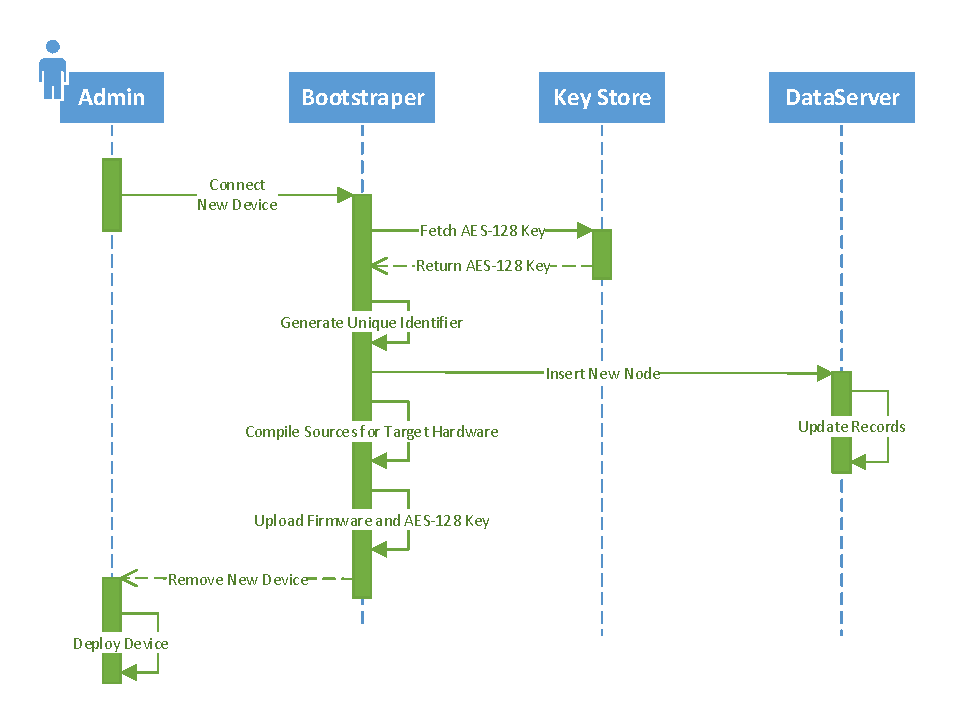
\includegraphics[width=0.95\linewidth]{figures/Sequence_Bootstrapping_Reviewed.pdf}
  \caption{Processo de \textit{Bootstrapping}}
  \label{fig:bootstrapping_process}
\end{figure}

\subsection{Arquitetura do Sistema}
\label{sec:system_architecture}
A inovação contida neste proposta advém dos outros dois componentes do sistema, o \textit{CoAP Client Observer}, e o \textit{Bootstrapper} que faz por sua vez uso de um \textit{Key Store}. 
O \textit{Key Store} é responsável por guardar a chave de rede utilizada no processo de \textit{bootstrapping}. 
O \textit{Bootstrapper} é responsável por conduzir o processo AutoStrap mapeando o novo dispositivo no sistema e fornecendo-lhe as credenciais de segurança necessárias. Por fim o \textit{CoAP Client Observer} atua como o único cliente da rede. Em vez de termos utilizadores a requisitar novas leituras diretamente aos sensores da rede com recursos limitados, este cliente regista-se junto dos dispositivos existentes e é notificado de cada novo valor ou evento despoletado pelos dispositivos. 

\section{Avaliação}
\label{sec:evaluation}
Primeiro, medimos e documentamos os recursos físicos necessários para suportar os protocolos e estratégias de mitigação escolhidas de forma a entender se são adequados ao \textit{hardware} usado na \ac{IdC}. Segundo, conduzimos testes de usabilidade ao nosso sistema de gestão de redes para analisar a sua eficiência e facilidade de uso.

\subsection{Aplicabilidade ao \textit{Hardware}}

Analisando os resultados podemos verificar que a introdução destes mecanismos comporta um aumento de 3.02\% na utilização de memória \textit{flash} e 1.02\% na utilização de memória \ac{RAM}, permitindo-nos concluir que apenas uma pequena fração de memória adicional é usada, o que nos parece um bom resultado.

Para entender se o tamanho de \textit{firmware} usado pelo nosso sistema é adequado aos dispositivos da \ac{IdC} foram analisadas três placas de desenvolvimento (Zolertia RE-Mote\footnote{http://zolertia.io/product/hardware/re-mote}, Arago Systems Wismote\footnote{http://www.wismote.com} e Texas Instruments CC2538DK\footnote{http://http://www.ti.com/tool/cc2538dk})


\begin{table}
\parbox{.45\linewidth}{
\centering
\caption{Consumos Energéticos}
\label{tab:power_consumptions}
\begin{tabular}{|l|c|c|c|} \hline
Modo&V&mA&W\\ \hline
Radio ON& 9.0& 17&0.15\\ \hline
Radio OFF& 9.0& 5.2&0.05\\ 
\hline\end{tabular}
}
\hfill
\parbox{.55\linewidth}{
\centering
\caption{Tempos de Bootstrapping}
\label{tab:bootstrapping_time}
\begin{tabular}{|l|c|} \hline
Operação&Tempo(s)\\ \hline
Inserir Novo Dispositivo&\,\,2\\ \hline
Abrir Interface&\,\,5\\ \hline
Selecionar Hardware&\,\,4\\ \hline
Compilar Código Fonte&13\\ \hline
Eliminar Firmware Existente&\,\,5\\ \hline
Upload Novo Firmware&\,\,3\\ \hline
Remover Novo Dispositivo&\,\,2\\ 
\hline\end{tabular}
}
\end{table}

\subsection{Processo de Bootstrapping}
Nesse caso, após a primeira sequência todo o processo de abertura da interface, seleção de \textit{hardware} e compilação já está realizado, representando um ganho de 22 segundos resultando num tempo real de 12 segundos. 
Desta forma podemos concluir que a nossa solução é prática e adequada aos cenários \ac{IdC}.

\section{Conclusões}
\label{sec:conclusion}
Obter comunicações seguras não é uma tarefa fácil, dadas as limitações dos dispositivos utilizados na redes \ac{IdC}. 
Para atingir este objetivo realizámos uma análise extensiva aos protocolos e estratégias de mitigação de ataques ``vampiros'' existentes estabelecendo uma pilha de protocolos que usámos nos dispositivos com recursos limitados. 
Experiências em \textit{hardware} real confirmam que 
%o \textit{stack} encontrado 
a solução tem tanto um tamanho como um consumo energético compatível com os dispositivos \ac{IdC}.
Face às exigências adicionais em termos de infraestrutura que o nosso modelo de comunicação necessita, propusemos uma arquitetura central que vai de encontro às necessidades correntes dos ambientes \ac{IdC} abordados e emprega mecanismos ao nível aplicacional para reduzir o número de pacotes que fluem na rede. 
Esta infraestrutura possui também os componentes adicionais de baixo impacto em termos de recursos necessários que permitem a execução do processo de \textit{bootstrapping} seguro proposto, 
automático, que não necessita de conhecimento interno por parte do operador e com métricas de usabilidade que o tornam adequado aos ambientes \ac{IdC}.

Como trabalho futuro, salientamos a necessidade de proteção da memória dos dispositivos para impedir o roubo de credenciais de segurança e consequente clonagem dos dispositivos. Deixamos como sugestão o uso de circuitos integrados com mecanismos de impedimento de leitura ou o bloqueio via software de certas regiões de memória dos dispositivos onde residem as chaves de rede.
%
% ---- Bibliography ----

\bibliographystyle{splncs}
\bibliography{references}

% *** DEFINITION OF ACRONYMS ***
\acrodef{IST}{Instituto Superior T\'ecnico}
\acrodef{IoT}{Internet of Things}
\acrodef{IdC}{Internet das Coisas}
\acrodef{MQTT}{Message Queue Telemetry Transport}
\acrodef{MQTT-SN}{Message Queue Telemetry Transport for Sensor Networks}
\acrodef{CoAP}{Constrained Application Protocol}
\acrodef{HTTP}{Hypertext Transfer Protocol}
\acrodef{TLS}{Transport Layer Security}
\acrodef{DTLS}{Datagram Transport Layer Security}
\acrodef{WWW}{World Wide Web}
\acrodef{MTU}{Maximum Transmission Unit}
\acrodef{TCP}{Transmission Control Protocol}
\acrodef{REST}{REpresentational State Transfer}
\acrodef{UDP}{User Datagram Protocol}
\acrodef{URIs}{Universal Resource Identifiers}
\acrodef{M2M}{Machine to Machine}
\acrodef{QoS}{Quality of Service}
\acrodef{WLAN}{Wireless Local Area Networks}
\acrodef{WPAN}{Wireless Private Area Networks}
\acrodef{LR-WPAN}{Low-Rate Wireless Private Area Networks}
\acrodef{MAC}{Medium Access Control}
\acrodef{FFD}{Full Function Device}
\acrodef{RFD}{Reduced Function Device}
\acrodef{IETF}{Internet Engineering Task Force}
\acrodef{DoS}{Denial of Service}
\acrodef{DODAG}{Destination Oriented Directed Acyclic Graph}
\acrodef{DIO}{DODAG Information Objects}
\acrodef{DAO}{Destination Advertisement Objects}
\acrodef{DIS}{DODAG Information Solicitation}
\acrodef{RFID}{Radio Frequency Identification}
\acrodef{ACL}{Access Control List}
\acrodef{6LoWPAN}{IPv6 over Low power Wireless Personal Area Networks}
\acrodef{RPL}{Routing Protocol for Low-Power and Lossy Networks}
\acrodef{CA}{Certificate Authority}
\acrodef{CSDS}{\ac{CoAP} Service Discovery Server}
\acrodef{RDC}{Radio Duty Cycling}
\acrodef{LLSec}{Link-Layer Security}
\acrodef{AES}{Advanced Encryption Standard}
\acrodef{CCM}{Counter with CBC-MAC}
\acrodef{MIC}{Message Integrity Code}
\acrodef{RAM}{Random-Access Memory}
\acrodef{OSI}{Open Systems Interconnection}
\end{document}
